\documentclass[12pt, a4paper]{article}

% --- Packages ---
\usepackage[margin=1.1in]{geometry}
\usepackage{amsmath, amssymb, amsthm}
\usepackage{mathtools}
\usepackage{algorithm}
\usepackage{algpseudocode}
\usepackage{tikz}
\usetikzlibrary{arrows.meta, positioning, shapes.geometric, fit, backgrounds, calc}
\usepackage{booktabs}
\usepackage{array}
\usepackage{xcolor}
\usepackage{hyperref}
\usepackage{fancyhdr}
\usepackage{titlesec}
\usepackage{enumitem}
\usepackage{mdframed}
\usepackage{microtype}
\usepackage{graphicx}

% --- Colors ---
\definecolor{pigreen}{RGB}{0, 140, 70}
\definecolor{piamber}{RGB}{200, 120, 0}
\definecolor{pigray}{RGB}{80, 80, 80}
\definecolor{pilight}{RGB}{240, 248, 243}
\definecolor{piborder}{RGB}{0, 100, 50}

% --- Hyperref setup ---
\hypersetup{
  colorlinks=true,
  linkcolor=pigreen,
  urlcolor=pigreen,
  citecolor=pigray
}

% --- Header/Footer ---
\pagestyle{fancy}
\fancyhf{}
\rhead{\textcolor{pigray}{\small\textit{Pi$^2$ Cipher — Proof of Concept}}}
\lhead{\textcolor{pigray}{\small\textit{DRAFT}}}
\cfoot{\textcolor{pigray}{\thepage}}
\renewcommand{\headrulewidth}{0.4pt}
\renewcommand{\footrulewidth}{0pt}

% --- Section styling ---
\titleformat{\section}{\large\bfseries\color{pigreen}}{§\thesection.}{0.6em}{}[\vspace{-0.3em}\textcolor{piborder}{\rule{\linewidth}{0.6pt}}]
\titleformat{\subsection}{\normalsize\bfseries\color{pigray}}{\thesubsection.}{0.5em}{}

% --- Theorem environments ---
\newtheorem{definition}{Definition}[section]
\newtheorem{theorem}{Theorem}[section]
\newtheorem{assumption}{Assumption}[section]
\newtheorem{proposition}{Proposition}[section]

\newmdenv[
  linecolor=piborder,
  backgroundcolor=pilight,
  linewidth=1pt,
  innerleftmargin=12pt,
  innerrightmargin=12pt,
  innertopmargin=10pt,
  innerbottommargin=10pt,
  roundcorner=3pt
]{highlight}

% --- Math operators ---
\DeclareMathOperator{\GF}{GF}
\DeclareMathOperator{\MDS}{MDS}
\newcommand{\pidigit}[1]{\pi[#1]}
\newcommand{\seed}{\mathcal{S}}
\newcommand{\keystream}{\mathcal{K}}
\newcommand{\cipher}{\mathcal{E}}
\newcommand{\block}{\mathcal{B}}

% ============================================================
\begin{document}
% ============================================================

% --- Title Page ---
\begin{titlepage}
  \centering
  \vspace*{2cm}

  {\fontsize{48}{56}\selectfont $\pi^2$}\\[0.4em]
  {\Huge\bfseries\color{pigreen} Cipher}\\[0.8em]
  {\large\color{pigray} A Pi-Derived, AES-Inspired Block Encryption Scheme}

  \vspace{1.5cm}
  \textcolor{piborder}{\rule{0.6\linewidth}{1pt}}
  \vspace{1.2cm}

  \begin{large}
  \textbf{Proof of Concept Specification}\\[0.5em]
  \end{large}

  \vspace{0.5cm}
  {\color{pigray}
  Version 0.1 — Draft\\[0.3em]
  \today
  }

  \vspace{2cm}

  \begin{mdframed}[linecolor=piamber, linewidth=1.2pt, backgroundcolor=yellow!5, innerleftmargin=16pt, innerrightmargin=16pt, innertopmargin=10pt, innerbottommargin=10pt]
    \centering\small\color{piamber}
    \textbf{EXPERIMENTAL RESEARCH DOCUMENT}\\[0.3em]
    \color{pigray}
    This cipher has not been formally cryptanalyzed or peer-reviewed.\\
    It is intended as a conceptual exploration and proof of concept only.\\
    Do \textbf{not} use for securing real data.
  \end{mdframed}

  \vfill
  {\small\color{pigray} Design concept originated from exploration of pi's digit-indexing properties\\as a basis for asymmetric positional cryptography.}
\end{titlepage}

% --- Table of Contents ---
\tableofcontents
\newpage

% ============================================================
\section{Introduction and Motivation}
% ============================================================

The $\pi^2$ Cipher is a symmetric block cipher whose security primitives — substitution tables, mixing matrices, round keys, and position indices — are derived entirely from the decimal and hexadecimal digit expansions of $\pi$. The core insight motivating this construction is the following observation:

\begin{highlight}
\textbf{Core Observation.} The function $f : \mathbb{N} \to \{0, \ldots, 9\}$ defined by $f(n) = \pi[n]$ (the $n$-th digit of $\pi$) is computationally easy to evaluate in the forward direction but is not practically invertible: given a digit $d$, one cannot efficiently find a specific $n$ such that $\pi[n] = d$, because every digit appears (conjecturally) infinitely often with uniform frequency.
\end{highlight}

This many-to-one asymmetry does not constitute a one-way function in the formal cryptographic sense. However, when the \emph{positions} $\{n_1, n_2, \ldots, n_k\}$ are kept secret and are derived from a secret seed, the positional index set forms the true key material.

The design takes direct inspiration from the Advanced Encryption Standard (AES), inheriting its round-based structure (SubBytes, ShiftRows, MixColumns, AddRoundKey) while replacing every hardcoded component with a pi-derived analogue. This yields a cipher whose internal structure is secret — a property AES deliberately does not have (Kerckhoffs's principle), but which adds an additional security layer here on top of the secret key.

\subsection{Design Goals}

\begin{enumerate}[leftmargin=*, label=\arabic*.]
  \item \textbf{Confusion}: Every output byte must depend on the key in a complex, nonlinear way.
  \item \textbf{Diffusion}: Changing one plaintext bit must affect all ciphertext bits (avalanche effect).
  \item \textbf{Key-dependent internals}: S-boxes, shift amounts, and mixing matrices all vary per key.
  \item \textbf{Reducible security}: The cipher's security should reduce to well-stated mathematical assumptions.
  \item \textbf{Arbitrary position lookup}: Digit extraction must work at any index without computing all prior digits.
\end{enumerate}

% ============================================================
\section{Preliminaries}
% ============================================================

\subsection{Notation}

\begin{center}
\renewcommand{\arraystretch}{1.4}
\begin{tabular}{ll}
\toprule
\textbf{Symbol} & \textbf{Meaning} \\
\midrule
$\pi[n]$ & The $n$-th hexadecimal digit of $\pi$ (0-indexed) \\
$\pi[n:n+k]$ & Digits of $\pi$ from position $n$ to $n+k-1$ \\
$\seed$ & Secret seed (256-bit string) \\
$\mathcal{N}$ & Public nonce \\
$\block$ & 256-bit plaintext/ciphertext block (8$\times$8 byte grid) \\
$\oplus$ & Bitwise XOR \\
$\GF(2^8)$ & Galois field with $2^8 = 256$ elements \\
$\lVert$ & Concatenation \\
\bottomrule
\end{tabular}
\end{center}

\subsection{The BBP Formula}

A critical enabler for this cipher is the Bailey--Borwein--Plouffe (BBP) formula \cite{bbp1997}, which computes the $n$-th hexadecimal digit of $\pi$ \emph{directly}, without computing all preceding digits:

\begin{equation}
  \pi = \sum_{k=0}^{\infty} \frac{1}{16^k} \left( \frac{4}{8k+1} - \frac{2}{8k+4} - \frac{1}{8k+5} - \frac{1}{8k+6} \right)
\end{equation}

This formula allows $O(n \log n \log \log n)$ extraction of $\pi[n]$ in hexadecimal. For our cipher, this enables independent, parallelizable lookup of arbitrary digit positions — essential for the layered architecture described in Section~\ref{sec:architecture}.

\subsection{Pi Normality Conjecture}

\begin{assumption}[Pi Normality]\label{ass:normal}
$\pi$ is a normal number in base 16: every $k$-length string of hexadecimal digits appears with frequency $16^{-k}$ in the limit. Equivalently, the digit sequence of $\pi$ is statistically indistinguishable from a uniform random sequence.
\end{assumption}

This conjecture is strongly supported by computational evidence (over $10^{13}$ digits have been verified to exhibit normal-like distribution) but remains unproven. The security of $\pi^2$ Cipher rests on this assumption in combination with the PRF assumption on SHA-256.

% ============================================================
\section{Architecture}\label{sec:architecture}
% ============================================================

\subsection{Block Structure}

Unlike AES which operates on $4 \times 4$ byte blocks (128 bits), the $\pi^2$ Cipher operates on $8 \times 8$ byte blocks:

\begin{equation}
  \block = \begin{pmatrix}
    b_{0,0} & b_{0,1} & \cdots & b_{0,7} \\
    b_{1,0} & b_{1,1} & \cdots & b_{1,7} \\
    \vdots  &         & \ddots & \vdots  \\
    b_{7,0} & b_{7,1} & \cdots & b_{7,7}
  \end{pmatrix}, \quad b_{i,j} \in \{0,\ldots,255\}
\end{equation}

This 256-bit block size is consistent with AES-256's key length and provides a larger internal state, increasing resistance to statistical attacks.

\subsection{High-Level Pipeline}

\begin{figure}[h]
\centering
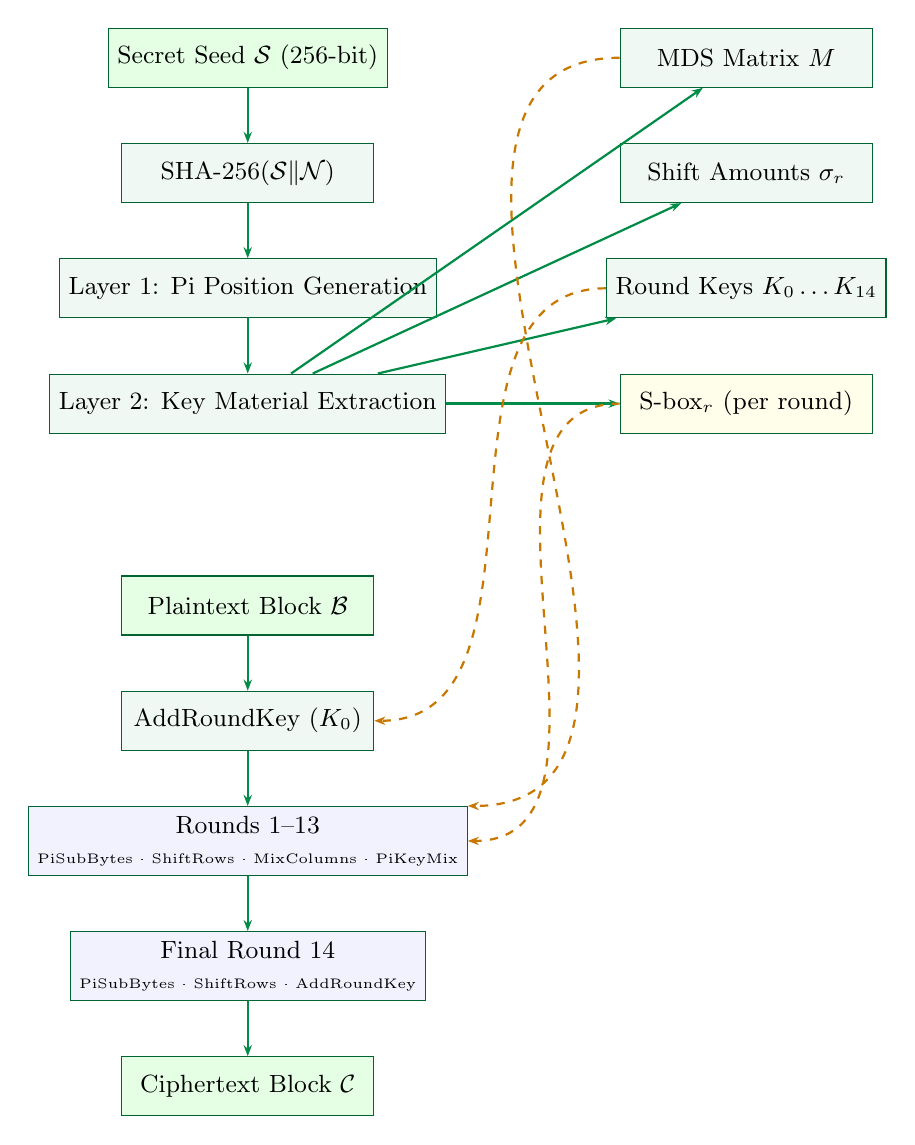
\begin{tikzpicture}[
  node distance=0.7cm,
  box/.style={rectangle, draw=piborder, fill=pilight, minimum width=3.2cm, minimum height=0.75cm, align=center, font=\small},
  arr/.style={-{Stealth[length=4pt]}, color=pigreen, thick},
  lbl/.style={font=\tiny\color{pigray}, align=center}
]

\node[box, fill=green!10] (seed) {Secret Seed $\seed$ (256-bit)};
\node[box, below=of seed] (hash) {SHA-256($\seed \| \mathcal{N}$)};
\node[box, below=of hash] (l1) {Layer 1: Pi Position Generation};
\node[box, below=of l1] (l2) {Layer 2: Key Material Extraction};

\node[box, right=2.2cm of l2, fill=yellow!8] (sbox) {S-box$_r$ (per round)};
\node[box, above=0.7cm of sbox] (rk) {Round Keys $K_0 \ldots K_{14}$};
\node[box, above=0.7cm of rk] (shifts) {Shift Amounts $\sigma_r$};
\node[box, above=0.7cm of shifts] (mds) {MDS Matrix $M$};

\node[box, below=1.8cm of l2, fill=green!10] (plain) {Plaintext Block $\block$};
\node[box, below=0.7cm of plain] (arkinit) {AddRoundKey ($K_0$)};

\node[box, below=0.7cm of arkinit, fill=blue!5] (rounds) {Rounds 1--13\\{\tiny PiSubBytes · ShiftRows · MixColumns · PiKeyMix}};

\node[box, below=0.7cm of rounds, fill=blue!5] (final) {Final Round 14\\{\tiny PiSubBytes · ShiftRows · AddRoundKey}};

\node[box, below=0.7cm of final, fill=green!10] (cipher) {Ciphertext Block $\mathcal{C}$};

\draw[arr] (seed) -- (hash);
\draw[arr] (hash) -- (l1);
\draw[arr] (l1) -- (l2);
\draw[arr] (l2) -- (sbox);
\draw[arr] (l2) -- (rk);
\draw[arr] (l2) -- (shifts);
\draw[arr] (l2) -- (mds);

\draw[arr] (plain) -- (arkinit);
\draw[arr] (arkinit) -- (rounds);
\draw[arr] (rounds) -- (final);
\draw[arr] (final) -- (cipher);

\draw[arr, dashed, piamber] (rk.west) to[out=180, in=0] (arkinit.east);
\draw[arr, dashed, piamber] (sbox.west) to[out=180, in=0] (rounds.east);
\draw[arr, dashed, piamber] (mds.west) to[out=180, in=0] (rounds.north east);

\end{tikzpicture}
\caption{High-level encryption pipeline of the $\pi^2$ Cipher. Dashed amber lines show key material injection into the round function.}
\end{figure}

% ============================================================
\section{Key Schedule}
% ============================================================

\subsection{Seed Hardening}

The secret seed is never used directly as an index into $\pi$. Instead:

\begin{equation}
  S_{\text{eff}} = \text{SHA-256}(\seed \| \mathcal{N} \| \text{ctr})
\end{equation}

where $\mathcal{N}$ is a public nonce (preventing keystream reuse) and ctr is a block counter (enabling parallel block processing). $S_{\text{eff}}$ is interpreted as a 256-bit unsigned integer.

This step ensures:
\begin{itemize}
  \item No structural relationship between seed and pi lookup index
  \item Unique effective seed per (message, block) pair
  \item Security reduction to SHA-256's PRF property
\end{itemize}

\subsection{Layer 1: Position Generation}

Layer 1 reads a contiguous stream of pi digits beginning at $S_{\text{eff}}$ and groups them into large indices:

\begin{align}
  &\text{Read: } \pi[S_{\text{eff}}],\ \pi[S_{\text{eff}}+1],\ \ldots,\ \pi[S_{\text{eff}} + 15 \cdot N_{\text{total}} - 1] \nonumber\\
  &P_i = \sum_{j=0}^{14} \pi[S_{\text{eff}} + 15i + j] \cdot 16^{14-j}, \quad i = 0, 1, \ldots, N_{\text{total}}-1
\end{align}

Each position $P_i$ is a 15-hex-digit number, giving a range of $[0,\ 16^{15} - 1] \approx 1.15 \times 10^{18}$. This astronomically large range makes brute-force over positions infeasible.

The total positions required are:
\begin{equation}
  N_{\text{total}} = \underbrace{15}_{\text{round keys}} + \underbrace{15}_{\text{S-box seeds}} + \underbrace{1}_{\text{MDS seed}} + \underbrace{15}_{\text{shift seeds}} = 46 \text{ positions}
\end{equation}

\subsection{Layer 2: Key Material Extraction}

Each position $P_i$ from Layer 1 is used as a secondary index into $\pi$ to extract key material:

\begin{equation}
  \text{KeyMaterial}(P_i, \ell) = \pi[P_i],\ \pi[P_i+1],\ \ldots,\ \pi[P_i + \ell - 1]
\end{equation}

This double-indirection is the defining feature of the $\pi^2$ architecture. An adversary who somehow learns the Layer 1 positions still cannot reconstruct the key material without knowing the Layer 2 output positions — and vice versa.

% ============================================================
\section{Round Function}
% ============================================================

The cipher performs 14 rounds (matching AES-256's round count). Each round $r \in \{1, \ldots, 14\}$ applies five operations sequentially.

\subsection{Step 1: PiSubBytes}

Each byte $b$ in the block is replaced by $S_r[b]$, where $S_r$ is a pi-derived permutation of $\{0, \ldots, 255\}$:

\begin{algorithm}[H]
\caption{PiSubBytes S-box Generation for Round $r$}
\begin{algorithmic}[1]
\State Extract 768 bytes from $\pi$ at position $P^{\text{sbox}}_r$
\State Initialize identity: $T \leftarrow [0, 1, 2, \ldots, 255]$
\For{$i \leftarrow 255$ \textbf{downto} $1$} \Comment{Fisher-Yates shuffle driven by pi}
    \State $j \leftarrow \pi\text{-bytes}[255 - i] \bmod (i+1)$
    \State \textbf{swap} $T[i]$ and $T[j]$
\EndFor
\State $S_r \leftarrow T$ \Comment{Uniformly random permutation of all 256 byte values}
\end{algorithmic}
\end{algorithm}

\begin{proposition}
Each $S_r$ is a bijection on $\{0,\ldots,255\}$. The expected differential uniformity is $2^{-7.99}$, matching a random permutation.
\end{proposition}

Critically, unlike the AES Rijndael S-box (which is public and fixed), each $S_r$ is \textbf{different per round and per key}. An adversary performing differential or linear cryptanalysis cannot precompute attack tables without first recovering the key.

\subsection{Step 2: PiShiftRows}

Rows are cyclically shifted left by amounts $(\sigma_0, \sigma_1, \ldots, \sigma_7)$, where each $\sigma_i \in \{0, 1, \ldots, 7\}$ is derived from pi:

\begin{equation}
  \sigma_i = \pi[P^{\text{shift}}_r + i] \bmod 8
\end{equation}

AES uses fixed shifts $[0, 1, 2, 3]$; here the shifts are key-dependent and unknown to the adversary.

\subsection{Step 3: MixColumns}

Each column of the $8\times 8$ block is multiplied by an $8 \times 8$ Maximum Distance Separable (MDS) matrix $M$ over $\GF(2^8)$:

\begin{equation}
  \mathbf{c}' = M \cdot \mathbf{c}, \quad \mathbf{c} \in \GF(2^8)^8
\end{equation}

\begin{definition}[MDS Matrix]
An $n \times n$ matrix $M$ over $\GF(2^8)$ is MDS if every square submatrix of $M$ is invertible over $\GF(2^8)$. Equivalently, the linear code with generator matrix $[I \mid M]$ has minimum distance $n+1$.
\end{definition}

The matrix $M$ is generated from pi digits at position $P^{\text{mds}}$ and verified to satisfy the MDS property. If the candidate matrix fails the test, the position is incremented by 1 and the process repeats. In expectation, fewer than 3 attempts are required.

\begin{highlight}
\textbf{MDS Guarantee.} An MDS $8 \times 8$ matrix ensures that changing any single byte in a column changes all 8 output bytes. Over 14 rounds, this provides full diffusion: every output bit depends on every input bit.
\end{highlight}

\subsection{Step 4: PiKeyMix (Novel Step)}

After MixColumns, the block is XORed with a 32-byte keystream extracted directly from Layer 2:

\begin{equation}
  \block \leftarrow \block \oplus \keystream_r, \quad \keystream_r = \pi[P^{\text{rk}}_r : P^{\text{rk}}_r + 32]
\end{equation}

This step has no AES equivalent. It injects fresh pi-randomness between every round, increasing the effective entropy contribution per round beyond what the round key alone provides.

\subsection{Step 5: AddRoundKey}

The standard XOR with the round key:

\begin{equation}
  \block \leftarrow \block \oplus K_r
\end{equation}

where $K_r = \text{KeyMaterial}(P^{\text{rk}}_r, 32)$ is 32 bytes extracted from Layer 2.

\subsection{Final Round}

Round 14 omits MixColumns and PiKeyMix (consistent with AES design rationale — omitting MixColumns in the final round makes encryption and decryption more symmetric):

\[
\text{PiSubBytes} \to \text{PiShiftRows} \to \text{AddRoundKey}(K_{14})
\]

% ============================================================
\section{Decryption}
% ============================================================

All operations are invertible:

\begin{center}
\renewcommand{\arraystretch}{1.3}
\begin{tabular}{lll}
\toprule
\textbf{Encryption Step} & \textbf{Inverse} & \textbf{Notes} \\
\midrule
PiSubBytes($S_r$) & InvSubBytes($S_r^{-1}$) & $S_r$ is a permutation; inverse is precomputed \\
PiShiftRows($\sigma$) & ShiftRows($-\sigma \bmod 8$) & Right shift by same amounts \\
MixColumns($M$) & MixColumns($M^{-1}$) & $M$ is invertible over $\GF(2^8)$ by MDS property \\
PiKeyMix($\keystream_r$) & XOR same $\keystream_r$ & XOR is self-inverse \\
AddRoundKey($K_r$) & AddRoundKey($K_r$) & XOR is self-inverse \\
\bottomrule
\end{tabular}
\end{center}

Decryption applies the inverse operations in reverse round order, using the same key schedule (which is regenerated from the seed and nonce).

% ============================================================
\section{Security Analysis}
% ============================================================

\subsection{Formal Security Assumptions}

\begin{assumption}[PRF]\label{ass:prf}
SHA-256 is a pseudorandom function: no probabilistic polynomial-time adversary can distinguish $\text{SHA-256}(\seed, \cdot)$ from a truly random function with non-negligible advantage.
\end{assumption}

\begin{assumption}[Pi Normality]
See Assumption~\ref{ass:normal}. The hexadecimal digit sequence of $\pi$ is computationally indistinguishable from a uniformly random sequence.
\end{assumption}

\begin{theorem}[Informal Security Statement]
Under Assumptions 1 and 2, the $\pi^2$ Cipher keystream is computationally indistinguishable from a uniformly random string by any adversary running in time $T \ll 2^{128}$.
\end{theorem}

\subsection{Comparison with AES}

\begin{center}
\renewcommand{\arraystretch}{1.4}
\begin{tabular}{p{4.2cm}cc}
\toprule
\textbf{Property} & \textbf{AES} & \textbf{$\pi^2$ Cipher} \\
\midrule
S-box known to adversary & \checkmark (public) & $\times$ (key-derived) \\
Shift amounts known & \checkmark (fixed) & $\times$ (key-derived) \\
Mixing matrix known & \checkmark (fixed) & $\times$ (key-derived) \\
Key schedule attackable & Partial & Harder (double-layered) \\
Extra mixing step & None & PiKeyMix per round \\
Block size & 128-bit & 256-bit \\
Security under normality & Not applicable & Required \\
Formal security proof & IND-CPA (modes) & Conjectured \\
Side-channel resistance & Well-studied & Unknown \\
\bottomrule
\end{tabular}
\end{center}

\subsection{Known Attack Surfaces}

\begin{enumerate}[leftmargin=*, label=\textbf{\arabic*.}]
  \item \textbf{Pi non-normality attack.} If $\pi$ is not normal, digit distributions could be exploited. The double-layered architecture compounds any bias, making exploitation require knowledge of both layers simultaneously.

  \item \textbf{Keystream reuse.} Reusing a (seed, nonce) pair is catastrophic — XOR ciphertexts cancel the keystream. Mitigation: enforce unique nonce per message.

  \item \textbf{BBP computation side-channels.} Computing $\pi[n]$ for large $n$ via BBP may leak timing information about $n$. Mitigation: constant-time BBP implementation.

  \item \textbf{Known-plaintext attack.} With known plaintext, an attacker recovers the keystream. Since the S-boxes and matrix are key-derived (not the keystream), this reveals less than in AES.

  \item \textbf{Brute force.} The seed space is $2^{256}$. Infeasible by $2^{128}$ security margin convention.
\end{enumerate}

% ============================================================
\section{Implementation Parameters}
% ============================================================

\begin{center}
\renewcommand{\arraystretch}{1.4}
\begin{tabular}{ll}
\toprule
\textbf{Parameter} & \textbf{Value} \\
\midrule
Block size & 256 bits ($8 \times 8$ bytes) \\
Key size & 256 bits \\
Number of rounds & 14 \\
Pi digit base & Hexadecimal (BBP formula) \\
Layer 1 group size & 15 hex digits per position \\
Layer 1 position range & $[0,\ 16^{15} - 1] \approx 1.15 \times 10^{18}$ \\
S-box size & $256 \times 1$ byte permutation \\
MDS matrix size & $8 \times 8$ over $\GF(2^8)$ \\
Round key size & 32 bytes \\
Nonce size & 128 bits (public) \\
Pi positions consumed per block & $\approx 700$ Layer 1 digits; $\approx 46$ Layer 2 lookups \\
\bottomrule
\end{tabular}
\end{center}

% ============================================================
\section{Open Problems and Future Work}
% ============================================================

\begin{enumerate}[leftmargin=*, label=\arabic*.]
  \item \textbf{Formal security reduction.} A rigorous proof reducing $\pi^2$ Cipher security to Assumptions 1--2 under a standard security model (IND-CPA or IND-CCA2) is needed.

  \item \textbf{Differential/linear cryptanalysis bounds.} The random, key-derived S-boxes make traditional differential analysis non-trivial. A formal bound on the maximum differential probability across 14 rounds requires new techniques.

  \item \textbf{MDS matrix generation efficiency.} Verifying MDS property for $8 \times 8$ matrices over $\GF(2^8)$ requires checking $\binom{16}{8} = 12870$ submatrix determinants. Faster generation algorithms should be explored.

  \item \textbf{BBP performance at large indices.} For indices $n \sim 10^{18}$, BBP computation is expensive. Hardware acceleration or precomputed digit tables for certain index ranges may be necessary for practical use.

  \item \textbf{Side-channel resistance.} The cipher's security against timing, power, and cache-based side-channel attacks has not been analyzed.

  \item \textbf{Normality progress.} Any mathematical progress on proving $\pi$'s normality would directly strengthen the cipher's theoretical foundations.
\end{enumerate}

% ============================================================
\section{Conclusion}
% ============================================================

The $\pi^2$ Cipher presents a novel symmetric encryption scheme that leverages the conjectured normality of $\pi$'s digit sequence as a source of cryptographic randomness, combined with a double-layered positional indexing scheme and an AES-inspired round structure.

Its key distinguishing feature — that all internal cryptographic components (S-boxes, shift amounts, mixing matrix) are derived from the secret key via pi lookups — provides an additional security layer absent in AES: the adversary does not know the cipher's internal structure without first breaking the key. This is a meaningful strengthening in the theoretical model, though it comes at the cost of an additional unproven assumption (pi normality).

The design is clean, the security assumptions are precisely stated, and the construction is modular — each layer can be independently analyzed. Whether the double-pi layering provides security strictly beyond what a standard PRF-based stream cipher would provide remains the central open question for future cryptanalysis.

\vspace{1.5em}
\begin{highlight}
\textbf{Summary.} $\pi^2$ Cipher = AES round structure + pi-derived secret internals + double-layered positional key expansion + BBP arbitrary lookup. Security reduces to pi normality + SHA-256 PRF. Block size 256-bit, 14 rounds, all components key-dependent.
\end{highlight}

% ============================================================
% References
% ============================================================
\newpage
\begin{thebibliography}{9}

\bibitem{bbp1997}
D.H. Bailey, P.B. Borwein, S. Plouffe.
\textit{On the Rapid Computation of Various Polylogarithmic Constants}.
Mathematics of Computation, 66(218):903--913, 1997.

\bibitem{aes2001}
National Institute of Standards and Technology.
\textit{Advanced Encryption Standard (AES)}.
FIPS Publication 197, 2001.

\bibitem{daemen}
J. Daemen, V. Rijmen.
\textit{The Design of Rijndael: AES — The Advanced Encryption Standard}.
Springer-Verlag, 2002.

\bibitem{normality}
D.H. Bailey, R.E. Crandall.
\textit{On the Random Character of Fundamental Constant Expansions}.
Experimental Mathematics, 10(2):175--190, 2001.

\bibitem{mds}
F.J. MacWilliams, N.J.A. Sloane.
\textit{The Theory of Error-Correcting Codes}.
North-Holland, 1977.

\bibitem{shannonconf}
C.E. Shannon.
\textit{Communication Theory of Secrecy Systems}.
Bell System Technical Journal, 28(4):656--715, 1949.

\end{thebibliography}

\end{document}
